\documentclass{article}
\usepackage[utf8]{inputenc}

\title{\textbf{Optimal low-thrust navigation around irregularly-shaped asteroids with DDP}}
\author{\textsc{Rory Lipkis}}
\date{}
\newcommand{\uvec}[1]{\boldsymbol{\hat{\textbf{#1}}}}
\newcommand{\conj}[1]{{#1}^{\dagger}}
\newcommand{\del}{\nabla}
\newcommand{\D}{\mathrm{d}}
\newcommand{\TD}[2]{\frac{d#1}{d#2}}
\newcommand{\TTD}[2]{\frac{d^{2}{#1}}{d{#2}^{2}}}
\newcommand{\PD}[2]{\frac{\partial#1}{\partial#2}}
\newcommand{\PPD}[2]{\frac{\partial^{2}{#1}}{\partial{#2}^{2}}}
\newcommand{\PPPD}[2]{\frac{\partial^{3}{#1}}{\partial{#2}^{3}}}
\newcommand{\la}{\langle}
\newcommand{\ra}{\rangle}
\newcommand{\const}[1]{\Big\rvert_{#1}}
\newcommand{\pfrac}[2]{\left(\frac{#1}{#2}\right)}
\usepackage{fullpage}
\usepackage{amsmath}
\usepackage{amssymb}
\usepackage{setspace}
\usepackage{mathtools}
\usepackage{enumerate}
\usepackage{esint}
\usepackage{booktabs}
\usepackage{physics}
\usepackage{siunitx}
\usepackage{graphicx}
\usepackage{graphics}
\usepackage{dsfont}
\usepackage{slashed}
\usepackage{multicol}
% \usepackage{float}

\begin{document}

\maketitle

\begin{multicols}{2}
\section*{Introduction}
As interest in asteroid exploration missions increases, there is use for low-thrust control around irregularly-shaped gravitating bodies. Recent missions to asteroids 67P/Churyumov–Gerasimenko (Rosetta) and 486958 Arrokoth (New Horizons) revealed bilobate shapes that cannot be easily navigated. Stacey and D'Amico 2018\footnote{Stacey, Nathan, and Simone D’Amico. ``Autonomous Swarming for Simultaneous Navigation and Asteroid Characterization.'' In \emph{AAS/AIAA Astrodynamics Specialist Conference}. 2018.} describe a method by which satellite formations could be used to estimate asteroid gravitational fields.

% \begin{figure}[H]
% 	\centering
% 	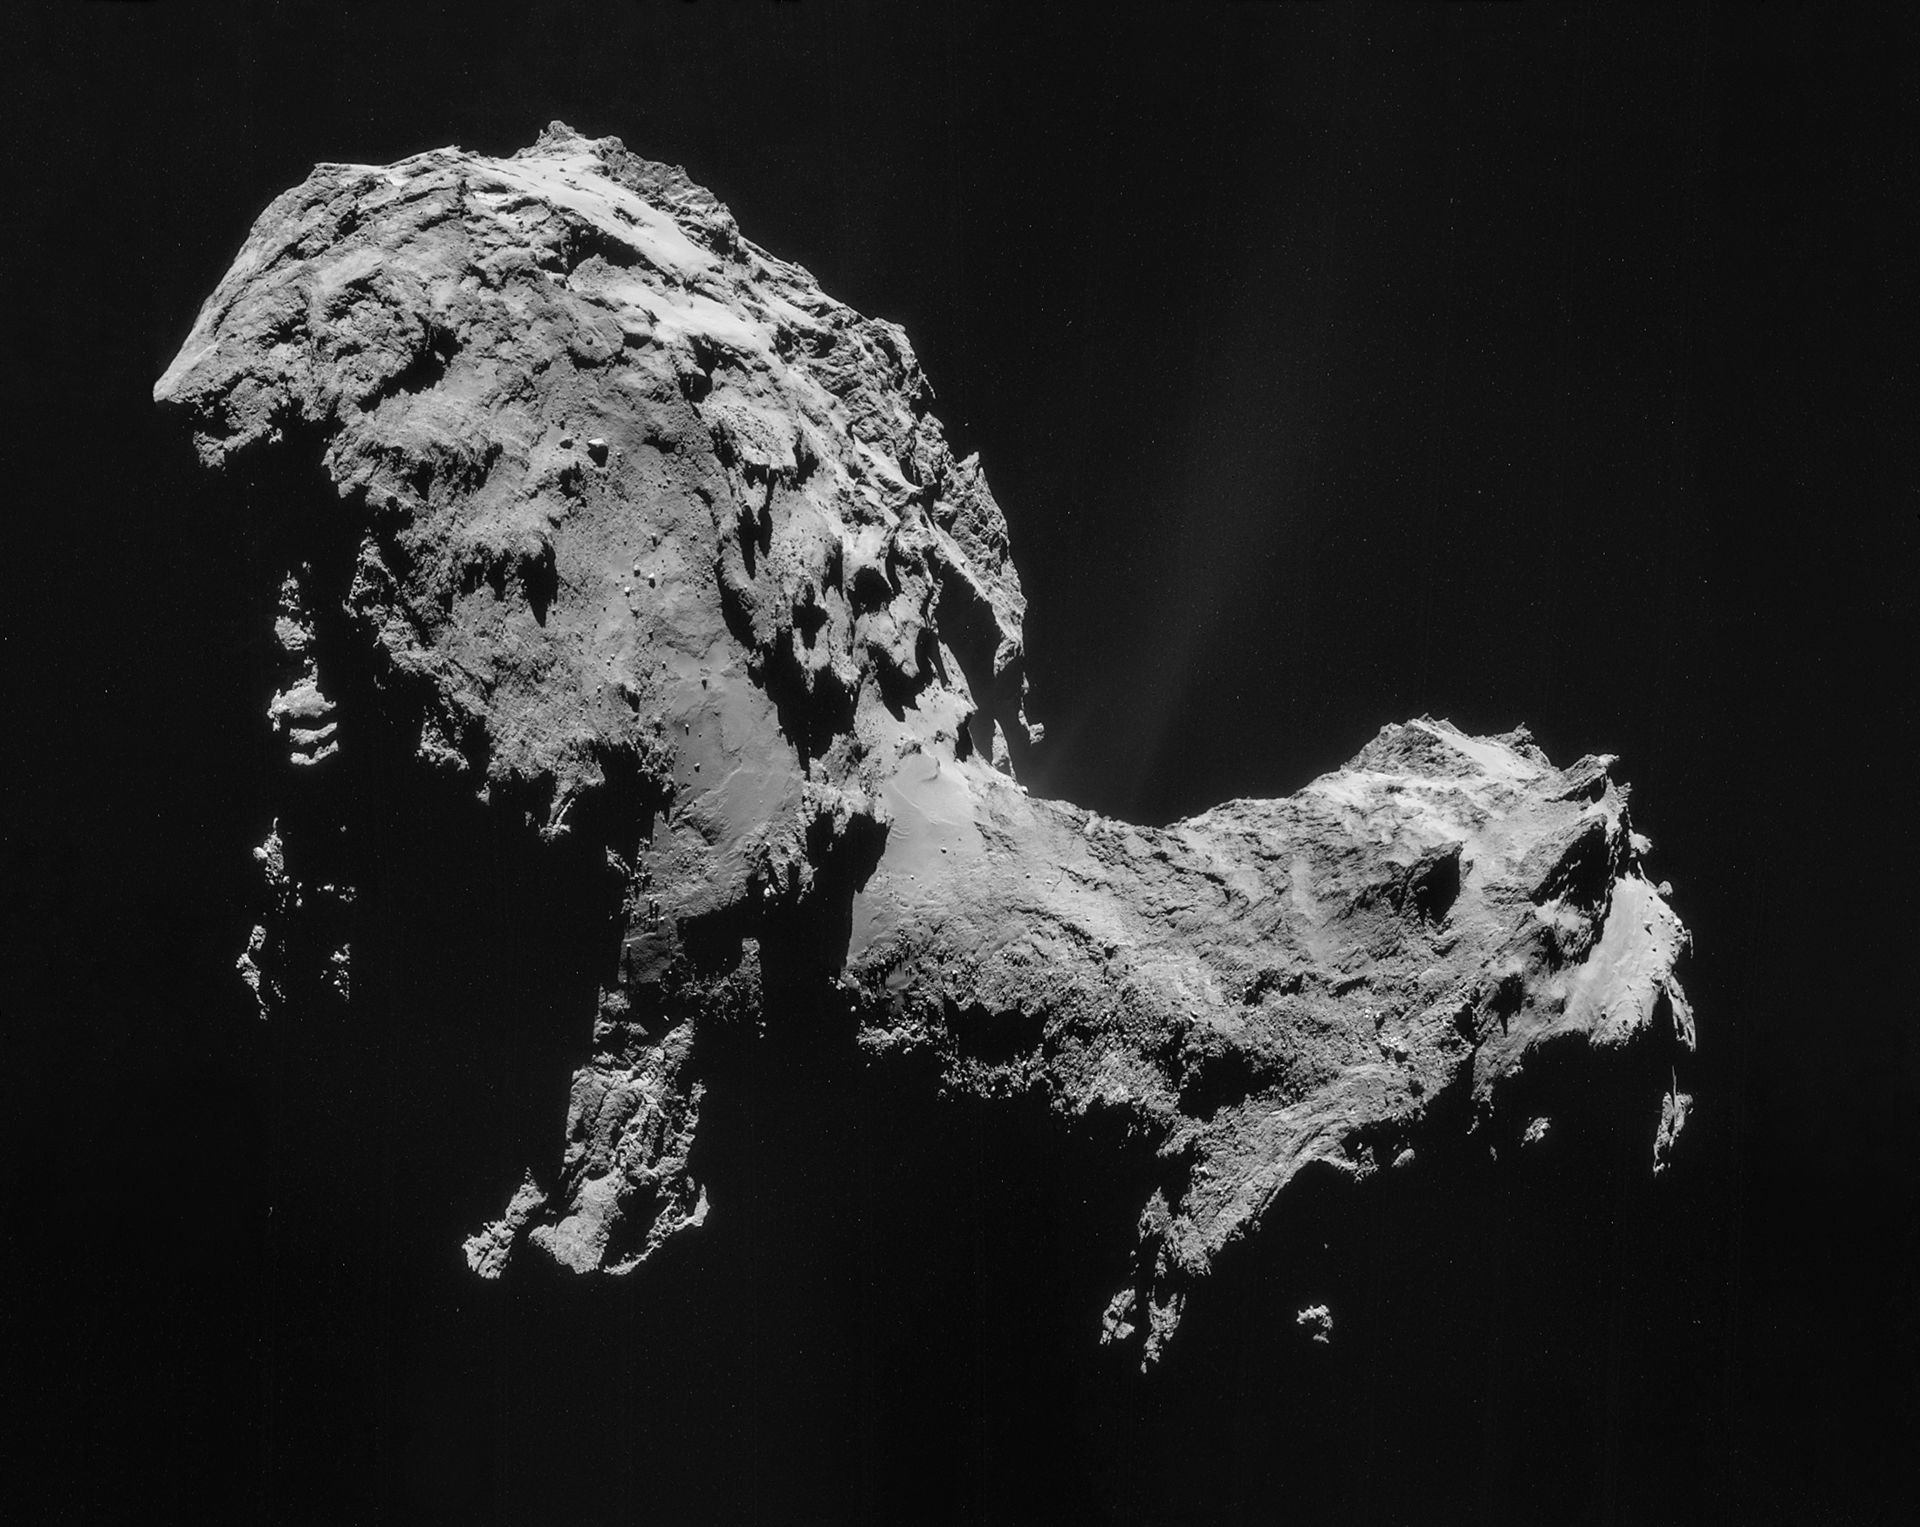
\includegraphics[width=0.8\linewidth]{comet}
% 	\caption{Comet 67P, via Wikipedia}
% \end{figure}

Nugnes and Colombo 2019\footnote{Nugnes, M., and C. Colombo. ``Low-thrust Trajectory Optimisation through Differential Dynamic Programming Method based on Keplerian Orbital Elements.'' In \emph{70th International Astronautical Congress (IAC 2019)}, pp. 1-9. 2019.} showed that a differential dynamic programming (DDP) approach could be successfully applied to the low-thrust control problem of orbital transfers around a spherical body. If the state is represented by non-dimensionalized orbital elements, the control inputs take the form of the Gauss variational equations. Since the orbital elements are constant for an unperturbed orbit (except for the mean anomaly, which can usually be ignored in the general problem of orbit transfer), the gravitational dynamics effectively disappear, and only the control inputs appear in the optimization. This allows for a concise representation of the system dynamics, which is handled easily by DDP.

Irregular gravitational fields are typically represented by their decomposition into spherical harmonics (the basis of Legendre polynomials). The orbital element representation can be modified to account for low-order harmonics, such as the $J2$ oblateness correction, with the introduction of mean and osculating elements, which specify an ``instantaneous'' unperturbed orbit. This would allow the aforementioned paper to be trivially extended to find optimal thrust solutions around slightly oblate bodies. Though useful for orbits around planets, this method does not generalize to trajectories in highly irregular gravitational fields, whose specifications require extremely high order spherical harmonics, and where the notion of orbital elements ceases to be useful. Since the trajectories are rarely stable orbits, they cannot be meaningfully specified by any set of dynamics-encapsulating elements, and the Cartesian position and velocity state must be used.
\section*{Problem and discussion}
\emph{For an asteroid with a highly irregular shape and gravitational field, use DDP to find optimal low-thrust control between any two position-velocity states. Demonstrate the control policy in a simulated mission that requires descending from a mother ship, visiting several locations on the surface of the asteroid, and returning to the mother ship.}

One challenge is that for an irregularly-shaped body, there are two spherical harmonic representations -- one which is valid only outside the circumscribing sphere, and one which is valid only within.\footnote{Takahashi, Yu, and D. J. Scheeres. ``Small body surface gravity fields via spherical harmonic expansions.'' \emph{Celestial Mechanics and Dynamical Astronomy} 119, no. 2 (2014): 169-206.} A general trajectory in the neighborhood of the body will require stitching together the two fields, which may cause convergence problems in a DDP approach. Generally, since orbital elements cannot be used, the gravitational dynamics must be specified explicitly. Fields close to an irregularly-shaped body can be highly nonlinear, and issues may arise with the second-order approximation that DDP uses. This is likely the most significant challenge of the project. One approach will be to sequentially increase the order of the spherical harmonic, using the output of the DDP convergence as the new initial guess.
\end{multicols}
\end{document}